\section{Examples}
\label{sec:examples}
In this section, the proposed method is applied to the two examples introduced in Section\ref{sec:preliminaries}.
The relaxed problems were constructed using the SPOTLESS toolbox \cite{spotless} and were numerically solved with MOSEK on a computer equipped with a Intel Xeon W3540 processor and 12GB of RAM.
Note that any set of probability distributions with identical support will generate the same uncertain backwards reachable set.
As a result it is assumed that the disturbance, $\theta$, is uniformly distributed.
For notional convenience, $\theta\sim\mathcal U([a,b])$ is used to denote that $\theta$ is uniformly distributed in the interval $[a,b]$.
Additionally during numerical implementation the state space in each problem is treated as the unit box in the appropriate dimension to avoid scaling problems.

\subsection{1-D Quasi-Uncertain Linear System}
Recall the 1-D linear dynamical system from Example \ref{example:1D} whose dynamics are:
  \begin{align}
	\dot x_1 = -0.7x_1+0.2\theta-0.1,
\label{eq:ex:1d}
\end{align}
where $\theta\in \mathcal U([0.2,1])$.
Setting $T = 1$ the target set is chosen as $X_T=[0.2,0.4]$.
If $\theta$ was a fixed constant then the backwards reachable set for a system evolving with this known constant the backwards reachable can be analytically computed as:
\begin{align}
	\begin{aligned}
  		BRS_\theta=&\left[\left(0.2-\frac{2\theta-1}{7}\right)e^{0.7}+\frac{2\theta-1}{7}, \right. \\
					&\hspace*{0.2cm}\left.\left(0.4-\frac{2\theta-1}{7}\right)e^{0.7}+\frac{2\theta-1}{7}\right]
	\end{aligned}
\end{align}
\normalsize
Note that the expression for the $BRS_\theta$ is linear in $\theta$ and that the width of $BRS_\theta$ is constant for all values of $\theta$.
As the value of $\theta$ changes, $BRS_\theta$ slides along $\R$; the intersection of $BRS_{0.2}$ and $BRS_1$ is the uncertain backwards reachable set of the system in Eqn.~(\ref{eq:ex:1d}) system.
\par
Fig.~\ref{fig:1D:linear} plots the degree 20 approximation of the $w_{20}$ that solves $D_{20}$ and the analytically computed indicator function supported on the BRS of the system, $\chi_{X_0}$. Observe that the 1-level superset of $w_{20}$ contains $X_{0}$ and hence is an outer approximation of $X_0$.
\begin{figure}[!t]
  {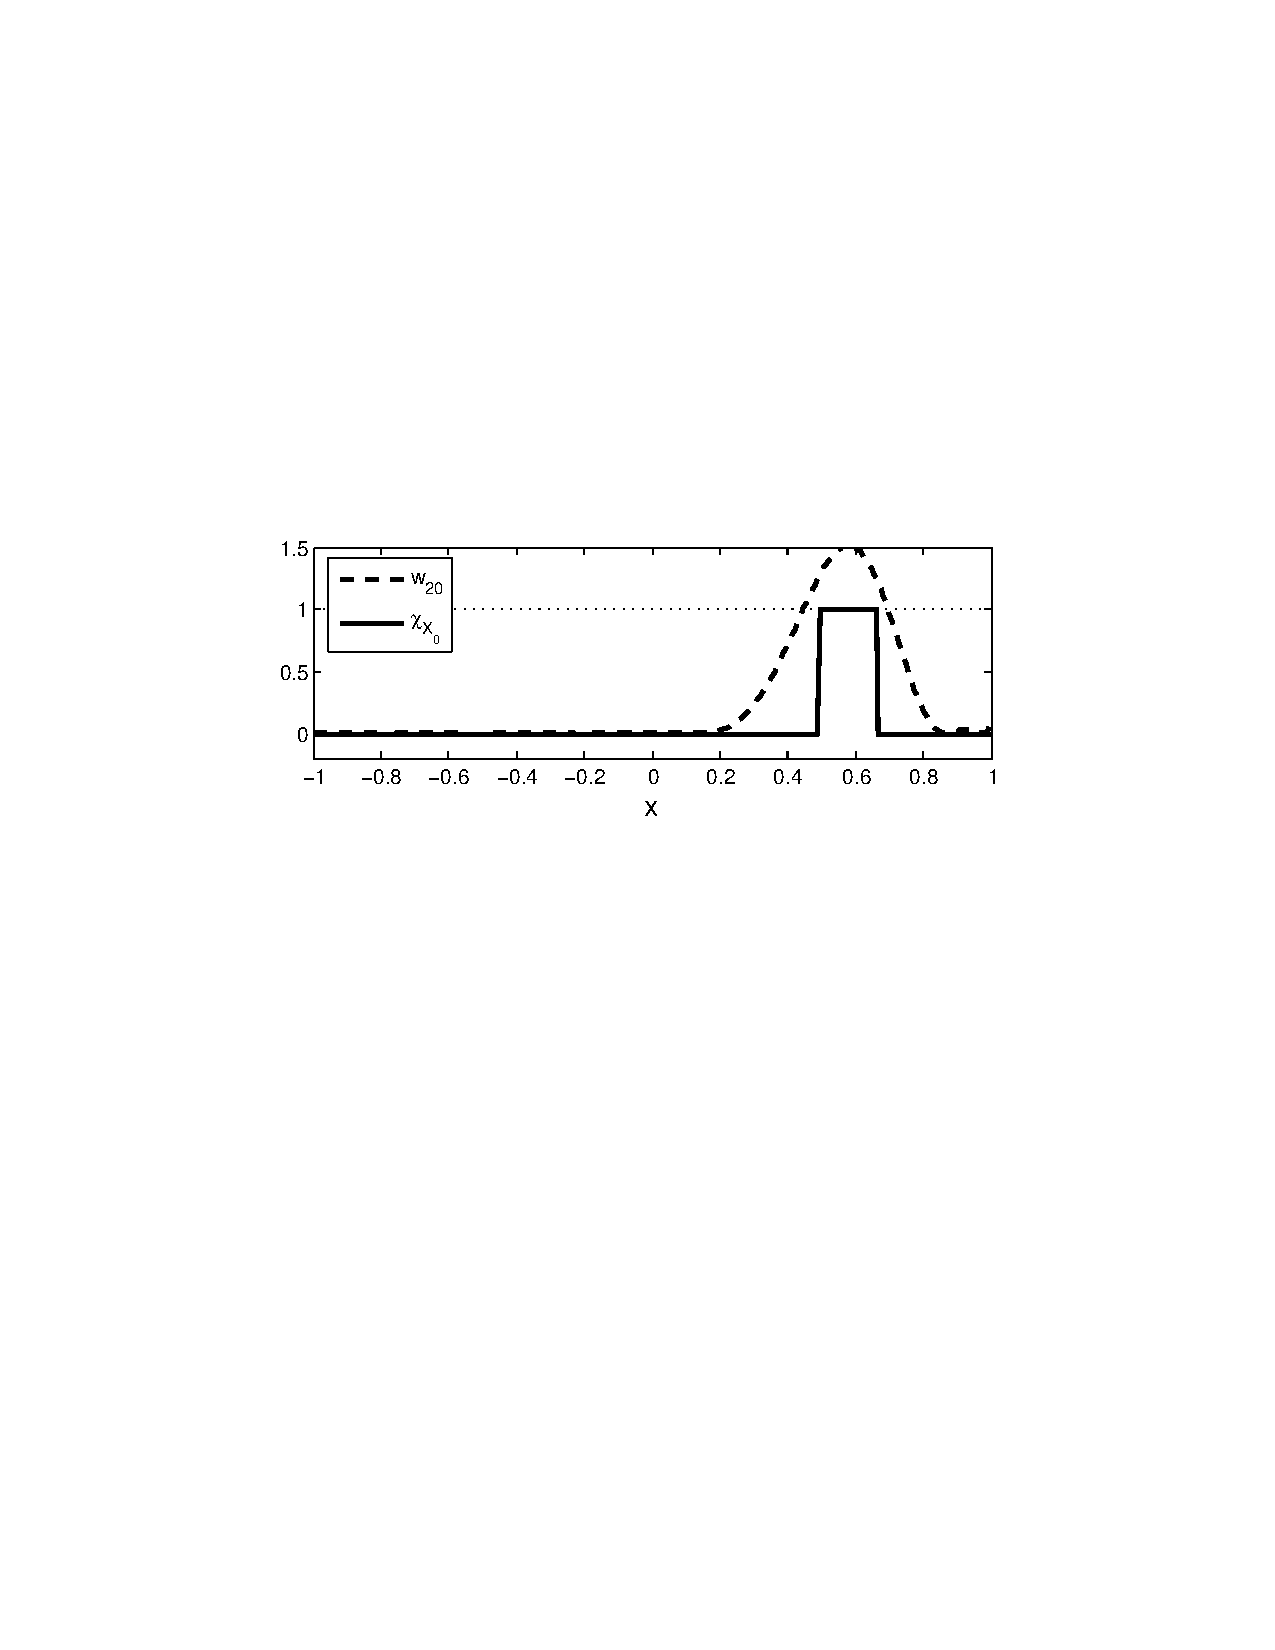
\includegraphics[width=\columnwidth,trim =1.5in 5.55in 1.5in 3.5in, clip=true]{figures/1D_ex_sp}}
  \caption{Outer approximation and the indicator function of the BRS}
    \label{fig:1D:linear}
\end{figure}
\subsection{Planar Rimless Wheel (PRW) with Uneven Terrain}
The PRW, introduced in Ex.\ref{example:rw}, is a one mode hybrid system in which the guard is reached when the swinging spoke makes contact with the inclined plane.
For a PRW rolling along an inclined plane with no terrain height variation (apart from the deterministic incline), an analytically computable stable limit cycle exits \cite{Coleman1998}; however, for the case considered in this example---with the inclined plane having variations in terrain height---the definition of a limit cycle is less clear.
Consequently, a notion of {\em meta-stability}---when the system states arrive within $\epsilon$ of the stable limit cycle of the disturbance-free system---is adopted.
\par
Fig.~\ref{fig:rw_brs} presents the polynomial degree 14 approximation to the uncertain backwards reachable set (black dashed) for the rimless wheel (with $\alpha=0.4$) which is tasked with arriving within the red band in $T=4$ seconds, as it is rolling down an inclined plane with slope $\gamma=0.2$. The terrain height, $\theta$, which affects the terrain height as described earlier in Ex.~\ref{example:rw} is allowed to drawn from a uniform distribution, $\theta\sim\mathcal U([-0.1,0.1])$. The maximum terrain variation is about 25\% the length of each spoke. With this setup, by the terminal time, the pivoting leg of the rimless wheel is likely to have changed between three and five times.
%\Ram{HOW many steps does this approximately correspond to?, How long does the optimization take? How long does MC take?}
\par
The approximate uncertain backwards reachable set is validated by performing Monte Carlo simulations; the unit box is discretized into 51 points in either direction and 100 independent trajectories are simulated (using MATLAB's {\em ode45} function) from each initial condition. The computation time of the MC simulation is 21019 seconds while the time to solve $D_{14}$ is 4487 seconds.
The blue $\cdot$s depict the initial conditions that arrived within the terminal set at the desired time without violating any of the other constraints. Note that the set of points that succeeded in the Monte Carlo simulation is entirely contained in the approximate uncertain backwards reachable set computed using our formulation. In fact, as a result of our method, we know that for points outside of the black region there exist a sequence of terrain heights that produce a trajectory that does not arrive at the target set.
\begin{figure}[!t]
  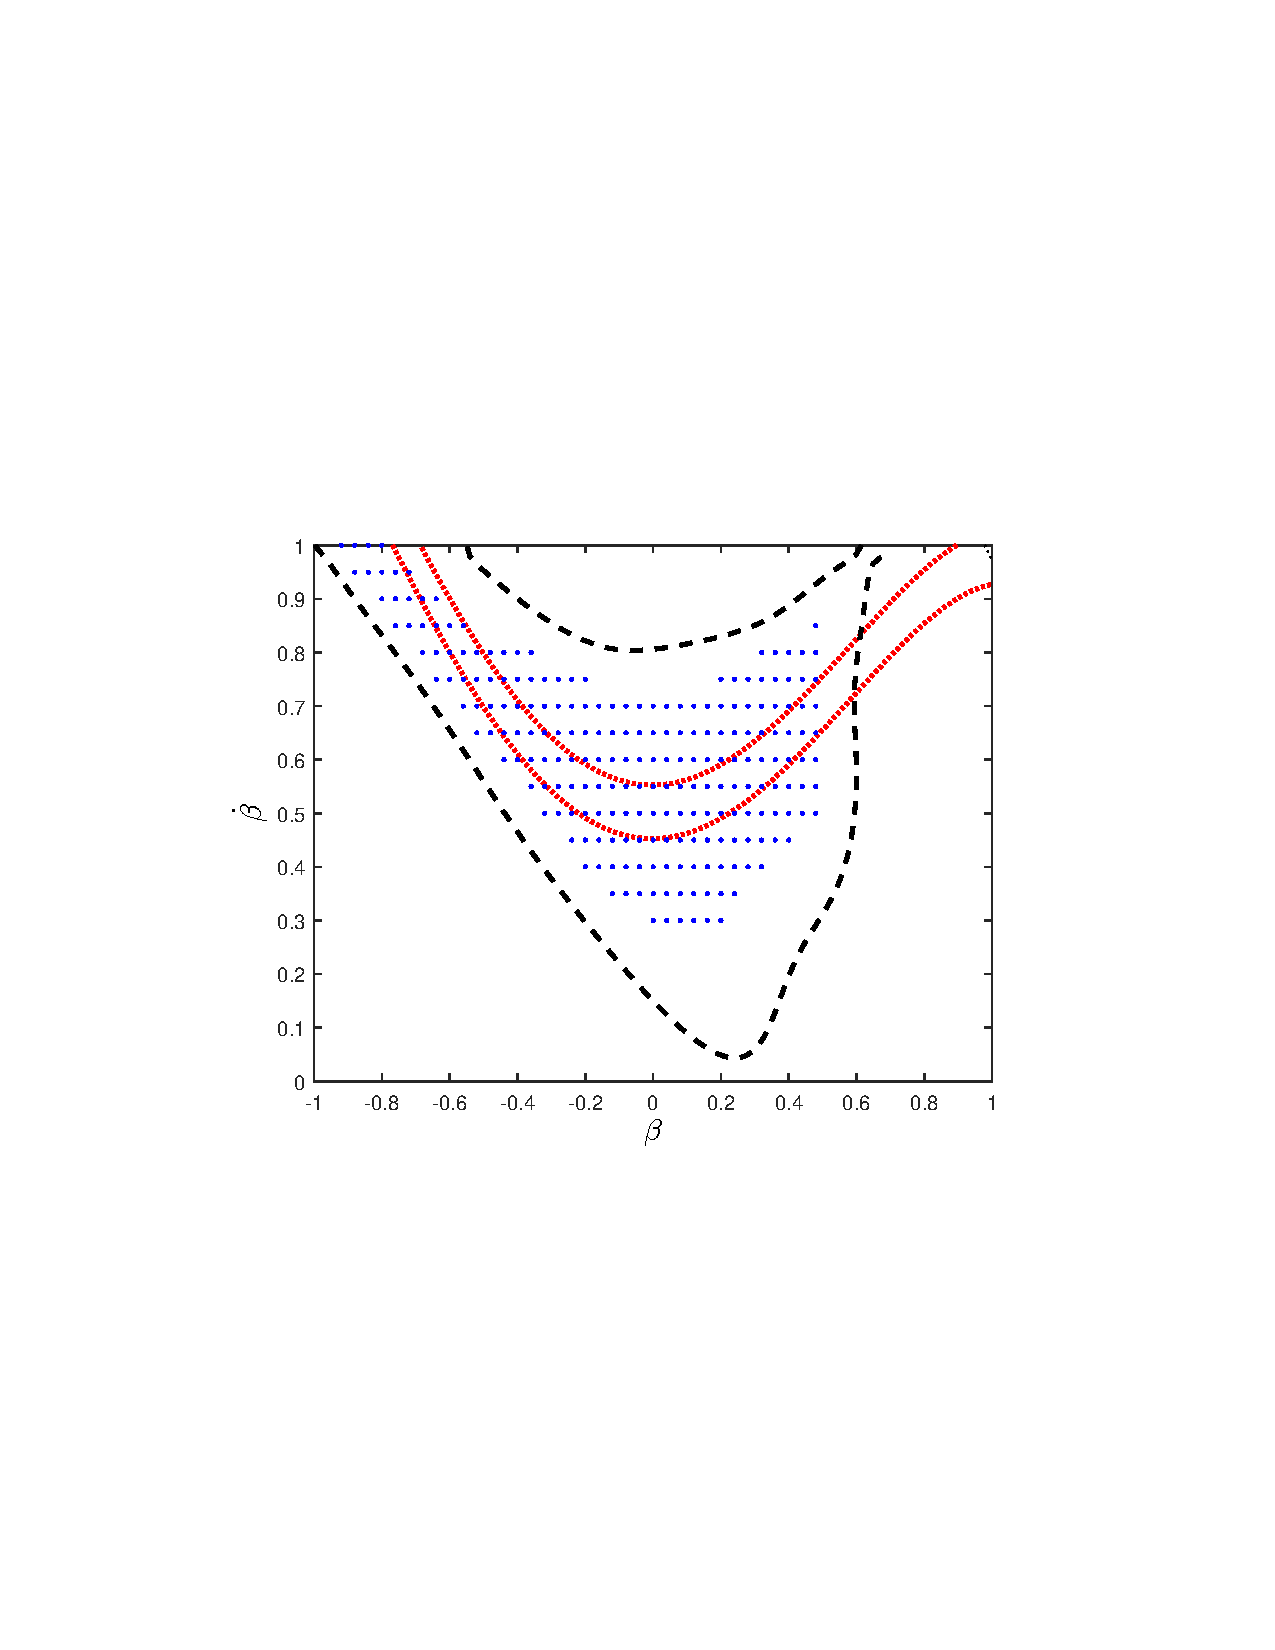
\includegraphics[trim=1.5in 3.3in 1.5in 3.5in, clip=true,width=\columnwidth]{figures/rw_0p1_4_new}
  \caption{Outer approximation and estimated BRS based on 100 iterations and T=4. Red band is the terminal set and the black outer is the boundary of the estimated BRS; the crosses correspond to results of MC simulation.}
  \label{fig:rw_brs}
\end{figure}
% At this juncture, a remark about the tightness of the BRS is warranted. Clearly, the BRS in Fig.~\ref{fig:rw_brs} is not tight; and we attribute this to the set of basis functions with which are currently working--monomials; and the degree relaxation. As commented in \cite{henrion2014convex}, adopting an alternate basis set is likely to increase the rate of convergence and the tightness. As it stands, there are alternate ways to improve the tightness, primary amongst which is to create phantom modes using identity reset maps; this approach however, needs some care and is deferred for a future work.
